%ch.tex


\chapter{An IO-monad for http streams}
\begin{center}
{\small\em Code first; questions later}
\end{center}

\begin{figure}[tbp]
\begin{center}
{ 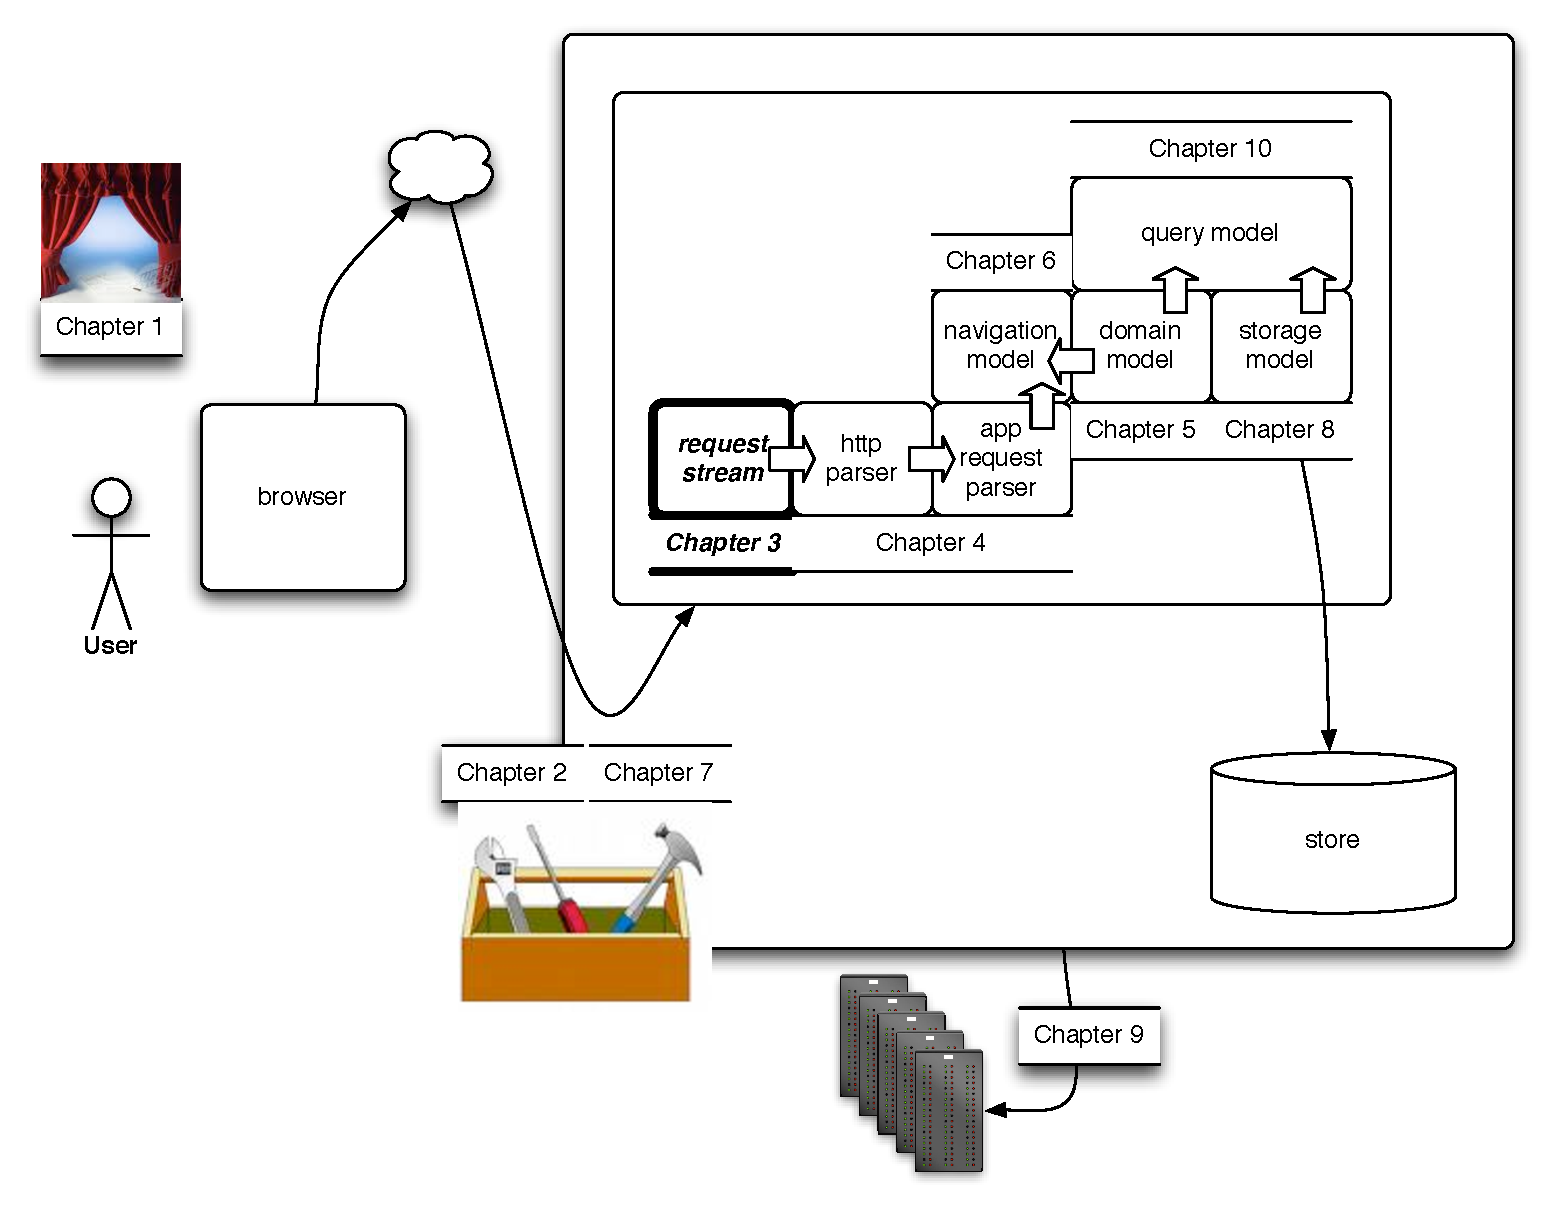
\includegraphics[scale=.35]{/Users/lgm/work/src/projex/biosimilarity/trace/src/main/book/content/figures/MonadicDesignPatternsChapterMapFocus3.pdf} }
\caption{ Chapter map }
\end{center}
\end{figure}

The following code is adapted from Tiark Rompf's work using delimited
continuations for handling HTTP streams.

\begin{figure}[tbp]
\begin{center}
{ 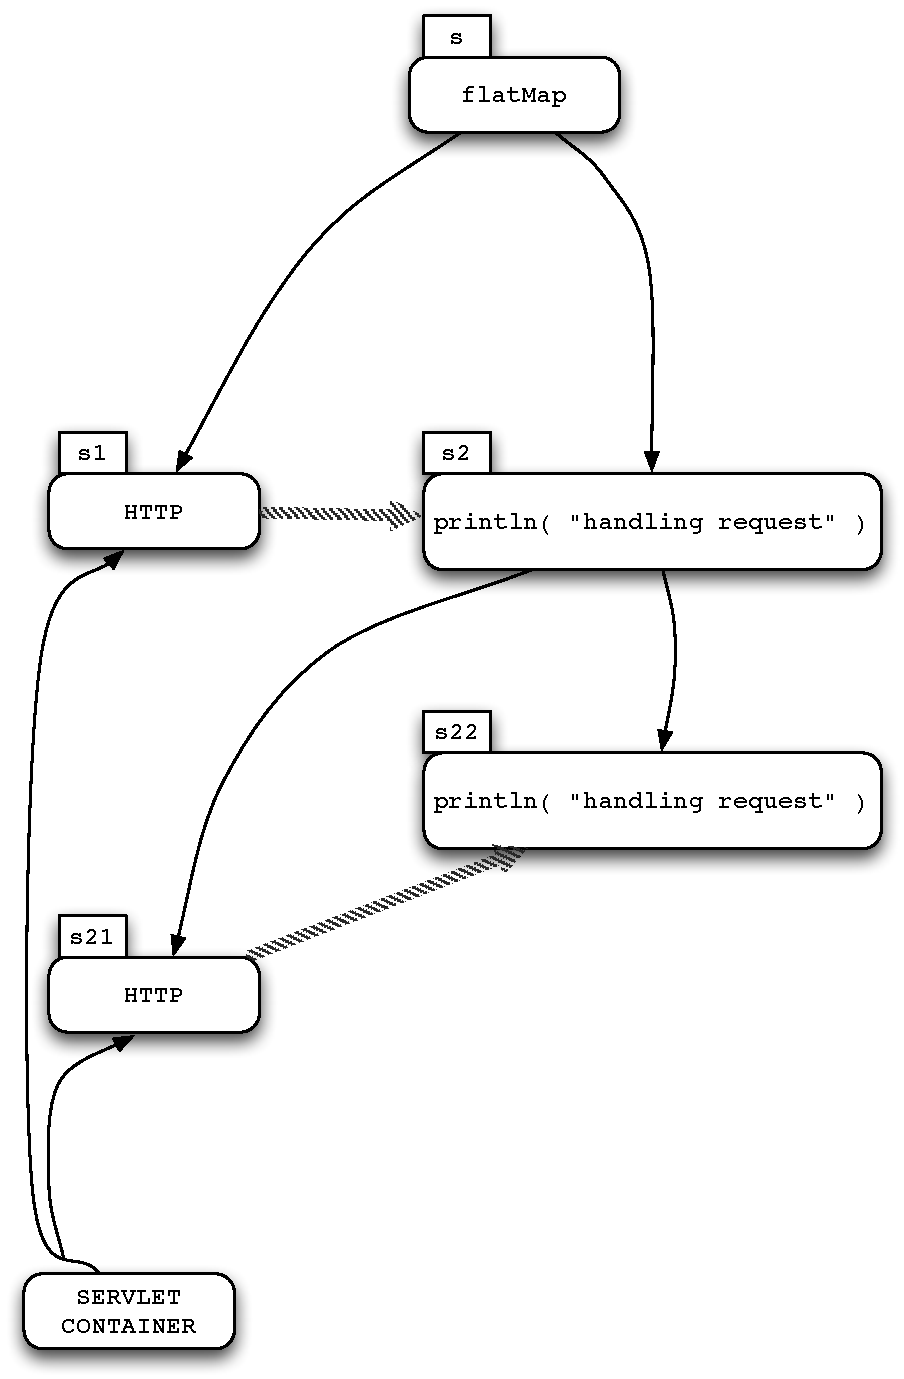
\includegraphics[scale=.85]{/Users/lgm/work/src/projex/biosimilarity/trace/src/main/book/content/figures/HTTPStreamExample0.pdf} }
\caption{ HTTP stream example 1 }
\end{center}
\end{figure}

\begin{figure}[tbp]
\begin{center}
{ 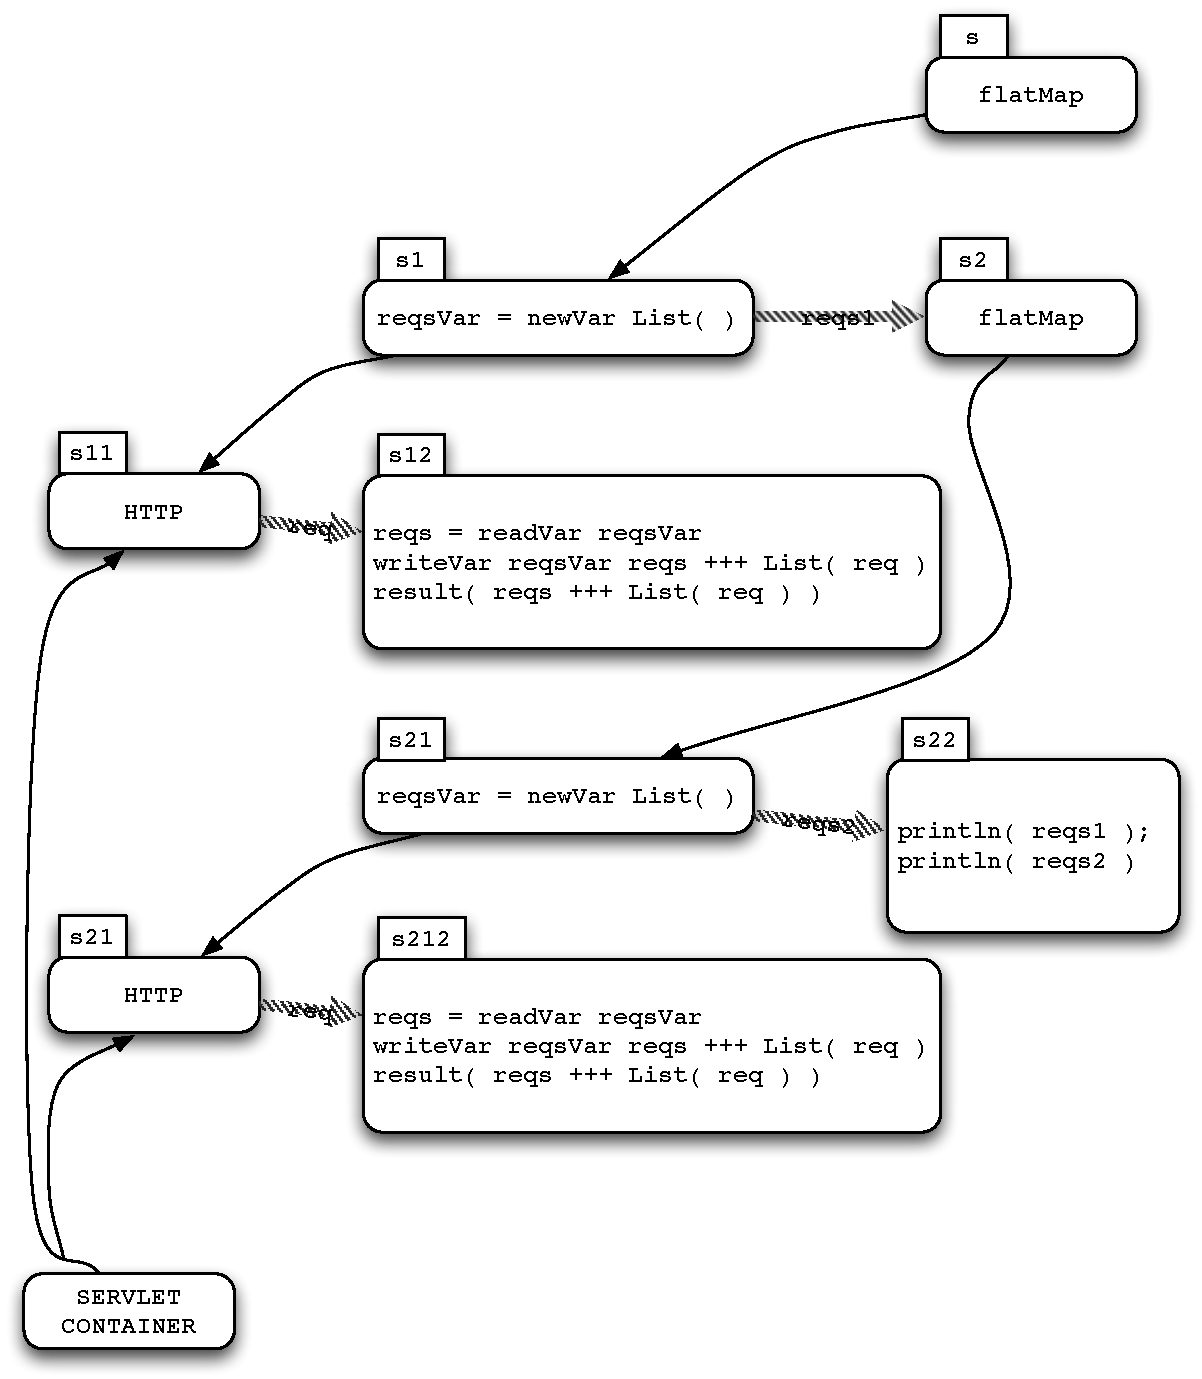
\includegraphics[scale=.85]{/Users/lgm/work/src/projex/biosimilarity/trace/src/main/book/content/figures/HTTPStreamExample1.pdf} }
\caption{ HTTP stream example 2 }
\end{center}
\end{figure}
\section{Code first, questions later}

\begin{lstlisting}[language=Scala]
import scala.continuations._
import scala.continuations.ControlContext._

import scala.concurrent._
import scala.concurrent.cpsops._


import java.net.InetSocketAddress
import java.net.InetAddress

import java.nio.channels.SelectionKey
import java.nio.channels.Selector
import java.nio.channels.SelectableChannel
import java.nio.channels.ServerSocketChannel
import java.nio.channels.SocketChannel
import java.nio.channels.spi.SelectorProvider

import java.nio.ByteBuffer
import java.nio.CharBuffer
import java.nio.charset.Charset
import java.nio.charset.CharsetDecoder
import java.nio.charset.CharsetEncoder

import java.util.regex.Pattern
import java.util.regex.Matcher

import java.util.Set

import scala.collection.JavaConversions._

// adapted from http://vodka.nachtlicht-media.de/tutHttpd.html

object DCWebserver
 extends FJTaskRunners {

  case class Generator[+A,-B,+C](val fun: (A => (B @cps[Any,Any])) => (C @cps[Any,Any])) {

    def copy = null // FIXME: workaround for named/default params bug

    final def foreach(f: (A => B @cps[Any,Any])): C @cps[Any,Any] = {
      fun(f)
    }
  }

  def selections( selector: Selector )
  : ControlContext[Set[SelectionKey], Unit, Unit] = 
  shiftR {
    k: (Set[SelectionKey] => Any) =>
      
    println("inside select")
	  
      while(true) { // problem???
        val count = selector.selectNow()
        if (count > 0)
          k(selector.selectedKeys())
      }
  }

  def createAsyncSelector() = {
    val selector = SelectorProvider.provider().openSelector()
	
    // TODO: this should run in its own thread, so select can block safely
    spawn {
      selections(selector).fun {
	keySet =>
  	  for (key <- keySet) {
    	    println("Select: " + key)	  
    	    val handler = key.attachment().asInstanceOf[(SelectionKey => Any)]
  	    
    	    println("handling: " + handler)
  	    handler(key)
    	  }
  	keySet.clear()
      }
    }

    selector
  }


  def callbacks(channel: SelectableChannel, selector: Selector, ops: Int) =
    Generator {
      k: (SelectionKey => Unit @cps[Any,Any]) =>
	println("level 1 callbacks")

      shift {
	outerk: (Unit => Any) =>

    	  def callback(key: SelectionKey) = {	  
    	    key.interestOps(0)
	    
    	    spawn { 
  	      println("before continuation in callback")
  	      
    	      k(key)
    	      
    	      println("after continuation in callback")
    	      
    	      if (key.isValid()) {
    		key.interestOps(ops)
    		selector.wakeup()
    	      } else {
    		outerk()
		//returnto.gen();
    	      }
    	    }
    	  }
  	     
  	println("before registering callback")
  	  
	val selectionKey = channel.register(selector, ops, callback _)
  	
  	println("after registering callback")
  	// stop
  	()
      }
    }

  def acceptConnections(selector: Selector, port: Int) =
    Generator {
      k: (SocketChannel => Unit @cps[Any,Any]) =>       
  	val serverSocketChannel = ServerSocketChannel.open()      
	serverSocketChannel.configureBlocking(false)
	
  	val isa = new InetSocketAddress(port)

  	serverSocketChannel.socket().bind(isa)
	
	for (
	  key <-
	  callbacks( serverSocketChannel, selector, SelectionKey.OP_ACCEPT )
	) {

    	  val serverSocketChannel =
	    key.channel().asInstanceOf[ServerSocketChannel]

  	  val socketChannel = serverSocketChannel.accept()
  	  socketChannel.configureBlocking(false)

	  k(socketChannel)
	}
      
      println("accept returning")
  }

  
  def readBytes(selector: Selector, socketChannel: SocketChannel) =
    Generator {
      k: (ByteBuffer => Unit @cps[Any,Any]) =>
	shift {
	  outerk: (Unit => Any) =>
	    reset {
	      val bufSize = 4096 // for example...
  	      val buffer = ByteBuffer.allocateDirect(bufSize)

	      println("about to read")

  	      for (
		key
		<- callbacks(
		  socketChannel, selector, SelectionKey.OP_READ
		)
	      ) {

		println("about to actually read")
        
  		val count = socketChannel.read(buffer)

  		if (count < 0) {
		  println("should close connection")
  		  socketChannel.close()
  				
  		  println("result of outerk " + outerk())
  		  //returnto.gen() should cancel here!
  		} else {

    		  buffer.flip()

		  println("about to call read cont")
		  
    		  k(buffer)
		  
  		  buffer.clear()
  		  shift { k: (Unit=>Any) => k() }
		}
  	      }
  	      
  	      println("readBytes returning")
  	      outerk()
	    }
  	}
    }
  

  def readRequests(selector: Selector, socketChannel: SocketChannel) =
    Generator {
      k: (String => Unit @cps[Any,Any]) =>
    
	var s: String = "";
    
	for ( buf <- readBytes( selector, socketChannel ) ) {
	  k("read: " + buf)
	}
    }


  def writeResponse(
    selector: Selector,
    socketChannel: SocketChannel,
    res: String
  ) = {
    val reply = res

    val charset = Charset.forName("ISO-8859-1")
    val encoder = charset.newEncoder()
    
    socketChannel.write(encoder.encode(CharBuffer.wrap(reply)))
  }


  def handleRequest(req: String) = req


  def test() = {

    val sel = createAsyncSelector()

    println("http daemon running...")

    for (socketChannel <- acceptConnections(sel, 8080)) {
      
      spawn {
    	println("Connect: " + socketChannel)

      	for (req <- readRequests(sel, socketChannel)) {

      	  val res = handleRequest(req)
		
      	  writeResponse(sel, socketChannel, res)
    	  
      	  shift { k: (Unit => Any) => k() } // FIXME: shouldn't be needed
      	}

    	println("Disconnect: " + socketChannel)
      }

      shift { k: (Unit => Any) => k() } // FIXME: shouldn't be needed
    }

  }



  // def main(args: Array[String]) = {
  
//     reset(test())

//     Thread.sleep(1000*60*60)  // 1h!
//     //    test.mainTaskRunner.waitUntilFinished()
  
//   }

}
\end{lstlisting}

\subsection{An HTTP-request processor}

\subsection{What we did}
\section{Synchrony, asynchrony and buffering}

TBD
\section{State, statelessness and continuations}

TBD

% \section{Existence problems}
% We begin with some metamathematics.
% All problems about the existence of maps can be cast into one of the
% following two forms, which are in a sense mutually dual.

% \noindent
% {\bf The Extension Problem}\index{extension problem} \    %%% NB index entry tag
% Given an inclusion $ A \stackrel{i}{\hookrightarrow} X $, and a map
% $ A \stackrel{f}{\rightarrow} Y $,
% does there exist a map $f^{\dagger}:X\to Y$ such that
% $f^{\dagger}$ agrees with $f$ on $A$?

% Here the appropriate source category for maps should be clear from the
% context and, moreover, commutativity through a
% candidate $f^{\dagger}$ is precisely
% the restriction requirement; that is,
% $$f^{\dagger}   :  f^{\dagger}\circ i = f^{\dagger}|_A = f\,. $$
% If such an $f^{\dagger}$ exists\footnote{${}^{\dagger}$ suggests striving
% for perfection, crusading}, then it is called an {\bf
% extension}\index{extension!of a map|bi} of $f$ and is said to {\bf
% extend}\index{extend|bi} $f$. In any diagrams, the presence of
% a dotted arrow or an arrow carrying a ? indicates a pious hope, in no way
% begging the question of its existence. Note that we shall usually
% omit $\circ$ from composite maps.

% \noindent
% {\bf The Lifting Problem}\index{lifting problem} \
% Given a pair of maps $E \stackrel{p}{\rightarrow}B$ and $X \stackrel{f}
% {\rightarrow} B $,
% does there exist a map $f^{\circ} : X \to E$, with
% $pf^{\circ} = f  $?


% That {\em all\/} existence problems about maps are essentially of one
% type or
% the other from these two is seen as follows. Evidently, all existence problems
% are representable by triangular diagrams\index{triangular diagrams} and it
% is easily seen that there are only these six possibilities:
% \begin{center}\begin{picture}(300,70)  %augch2 75
% \put(5,60){\vector(1,0){30}}
% \put(55,60){\vector(1,0){30}}
% \put(135,60){\vector(-1,0){30}}
% \put(185,60){\vector(-1,0){30}}
% \put(235,60){\vector(-1,0){30}}
% \put(285,60){\vector(-1,0){30}}
% \put(0,55){\vector(0,-1){30}}
% \put(50,55){\vector(0,-1){30}}
% \put(100,25){\vector(0,1){30}}
% \put(150,25){\vector(0,1){30}}
% \put(200,55){\vector(0,-1){30}}
% \put(250,55){\vector(0,-1){30}}
% \put(28,33){\small ?}
% \put(78,33){\small ?}
% \put(128,33){\small ?}
% \put(178,33){\small ?}
% \put(228,33){\small ?}
% \put(278,33){\small ?}
% \put(10,3){\bf 1}
% \put(60,3){\bf 2}
% \put(110,3){\bf 3}
% \put(160,3){\bf 4}
% \put(210,3){\bf 5}
% \put(260,3){\bf 6}
% \put(35,55){\vector(-1,-1){30}}
% \put(155,25){\vector(1,1){30}}
% \put(135,55){\vector(-1,-1){30}}
% \put(55,25){\vector(1,1){30}}
% \put(235,55){\vector(-1,-1){30}}
% \put(255,25){\vector(1,1){30}}
% \end{picture}\end{center}



% \begin{figure}
% \begin{picture}(300,220)(0,0)
% \put(-20,-20){\resizebox{20 cm}{!}{\includegraphics{3dpdf}}}
% \put(260,-10){\resizebox{15 cm}{!}{\includegraphics{contpdf}}}
% \put(220,80){$\beta$}
% \put(400,-10){$N$}
% \put(260,170){$\beta$}
% \put(90,15){$N$}
% \end{picture}
% \caption{{\em The log-gamma family of densities with central mean
% $<N> \, = \frac{1}{2}$ as a surface and as a contour plot. }}
% \label{pdf}
% \end{figure}

\newpage
